
\subsection{Number Formatting Options}
\label{sec:number:printing}%
\PGFPlots\ typeset tick labels rounded to given precision and in configurable number formats. The command to do so is |\pgfmathprintnumber|; it uses the current set of number formatting options.

These options are described in all detail in the manual for \PGFPlotstable, which comes with \PGFPlots. Please refer to that manual.

\begin{command}{\pgfmathprintnumber\marg{x}}
Generates pretty-printed output for the (real) number \marg{x}. The input number \marg{x} is parsed using |\pgfmathfloatparsenumber| which allows arbitrary precision.

Numbers are typeset in math mode using the current set of number printing options, see below. Optional arguments can also be provided using |\pgfmathprintnumber[|\meta{options}|]|\marg{x}.

Please refer to the manual of \PGFPlotstable\ (shipped with this package) for details about the number options.
\end{command}

\label{sec:identify:minor:log}%
\begin{pgfplotskey}{log identify minor tick positions=\mchoice{true,false} (initially false)}
Set this to |true| if you want to identify log--plot tick labels at positions 
\[ i \cdot 10^j \]
with $i \in \{2,3,4,5,6,7,8,9\},\, j \in \Z$. This may be valuable in conjunction with the `|extra x ticks|' and `|extra y ticks|' options.
\begin{codeexample}[]
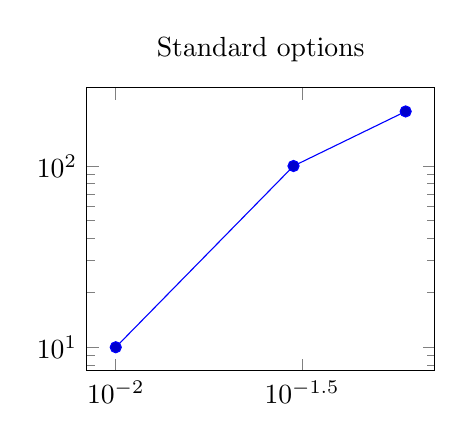
\begin{tikzpicture}%
\begin{loglogaxis}
	[title=Standard options,
	width=6cm]
\addplot coordinates {
	(1e-2,10)
	(3e-2,100)
	(6e-2,200)
};
\end{loglogaxis}
\end{tikzpicture}%
\end{codeexample}

\begin{codeexample}[]
\pgfplotsset{every axis/.append style={%
	width=6cm,
	xmin=7e-3,xmax=7e-2,
	extra x ticks={3e-2,6e-2},
	extra x tick style={major tick length=0pt,font=\footnotesize}
}}%

\begin{tikzpicture}%
	\begin{loglogaxis}[
		xtick={1e-2},
		title=with minor tick identification,
		extra x tick style={
			log identify minor tick positions=true}]
	\addplot coordinates {
		(1e-2,10)
		(3e-2,100)
		(6e-2,200)
	};
	\end{loglogaxis}
\end{tikzpicture}%

\begin{tikzpicture}%
	\begin{loglogaxis}[
		xtick={1e-2},
		title=without minor tick identification,
		extra x tick style={
			log identify minor tick positions=false}]
	\addplot coordinates {
		(1e-2,10)
		(3e-2,100)
		(6e-2,200)
	};
	\end{loglogaxis}%
\end{tikzpicture}%
\end{codeexample}
	This key is set by the default styles for extra ticks.
\end{pgfplotskey}

\begin{pgfplotscodekey}{log number format code}
Provides \TeX-code to generate log plot tick labels. Argument `|#1|' is the (natural) logarithm of the tick position.
The default implementation invokes |log base 10 number format code| after it changed the log basis to~$10$. It also checks the other log plot options.

This key will have a different meaning when the log basis has been chosen explicitly, see the |log basis x| key.
\end{pgfplotscodekey}


\begin{pgfplotscodekey}{log base 10 number format code}
Allows to change the overall appearance of base 10 log plot tick labels. The default is
\begin{codeexample}[code only]
\pgfplotsset{
	log base 10 number format code/.code={$10^{\pgfmathprintnumber{#1}}$}
}
\end{codeexample}
where the `|log plot exponent style|' allows to change number formatting options.
\end{pgfplotscodekey}

\begin{pgfplotscodekey}{log number format basis}
	This part of the representation routines for log ticks in \emph{arbitrary} basis (see the |log basis x| key). It is used instead of the key above if the log basis has been changed. The first supplied argument is the log basis, the second the exponent. The initial configuration is
\begin{codeexample}[code only]
\pgfplotsset{
	/pgfplots/log number format basis/.code 2 args={$#1^{\pgfmathprintnumber{#2}}$}
}
\end{codeexample}
\end{pgfplotscodekey}

\begin{pgfplotskey}{log plot exponent style=\marg{key-value-list}}
Allows to configure the number format of log plot exponents. This style is installed just before `|log base 10 number format code|' will be invoked. Please note that this style will be installed within the default code for `|log number format code|'.
\begin{codeexample}[]
\pgfplotsset{
	samples=15,
	width=7cm,
	xlabel=$x$,
	ylabel=$f(x)$,
	extra y ticks={45},
	legend style={at={(0.03,0.97)},
		anchor=north west}}

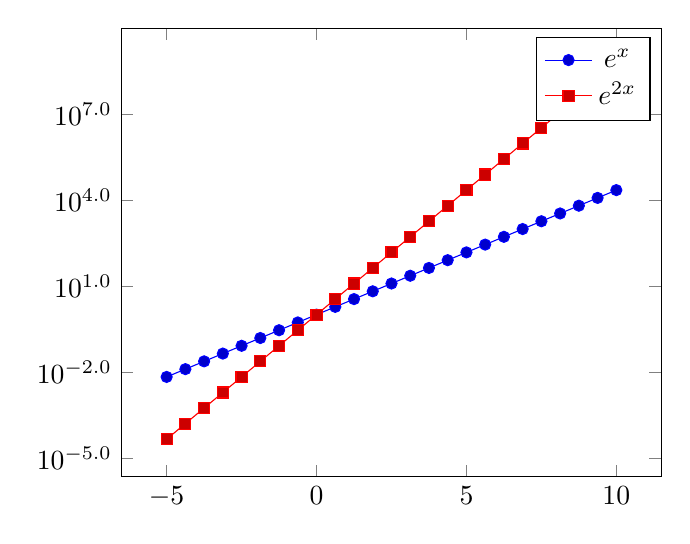
\begin{tikzpicture}
\begin{semilogyaxis}[
	log plot exponent style/.style={
		/pgf/number format/fixed zerofill,
		/pgf/number format/precision=1},
	domain=-5:10]

	\addplot {exp(x)};
	\addplot {exp(2*x)};

	\legend{$e^x$,$e^{2x}$}
\end{semilogyaxis}
\end{tikzpicture}
\end{codeexample}

\begin{codeexample}[]
\pgfplotsset{
	samples=15,
	width=7cm,
	xlabel=$x$,
	ylabel=$f(x)$,
	extra y ticks={45},
	legend style={at={(0.03,0.97)},
		anchor=north west}}

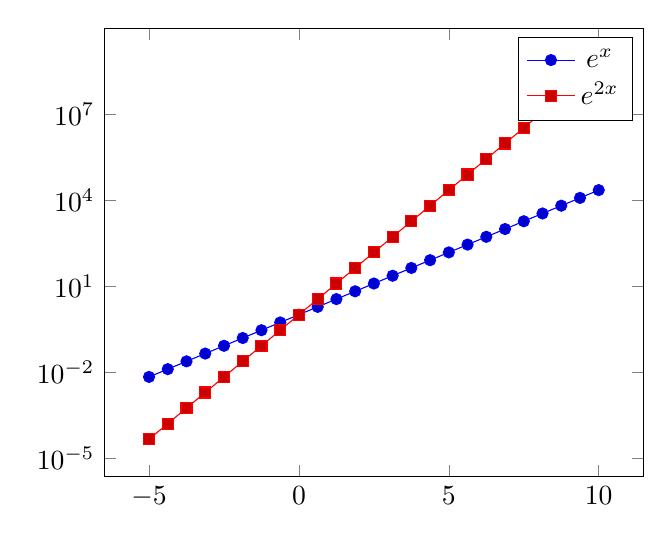
\begin{tikzpicture}
\begin{semilogyaxis}[
	log plot exponent style/.style={
		/pgf/number format/fixed,
		/pgf/number format/use comma,
		/pgf/number format/precision=2},
	domain=-5:10]

	\addplot {exp(x)};
	\addplot {exp(2*x)};

	\legend{$e^x$,$e^{2x}$}
\end{semilogyaxis}
\end{tikzpicture}
\end{codeexample}
\end{pgfplotskey}

